\begin{appendices}

%Some Table of Contents entry formatting
\addtocontents{toc}{\protect\renewcommand{\protect\cftchappresnum}{\appendixname\space}}
\addtocontents{toc}{\protect\renewcommand{\protect\cftchapnumwidth}{6em}}

%Begin individual appendices, separated as chapters
\chapter{PDT Background Questionnaire}
\label{appendix:questionnaire}
This section presents the brief background questionnaire given to participants of the picture description task discussed in Chapter~\ref{chap:data}.

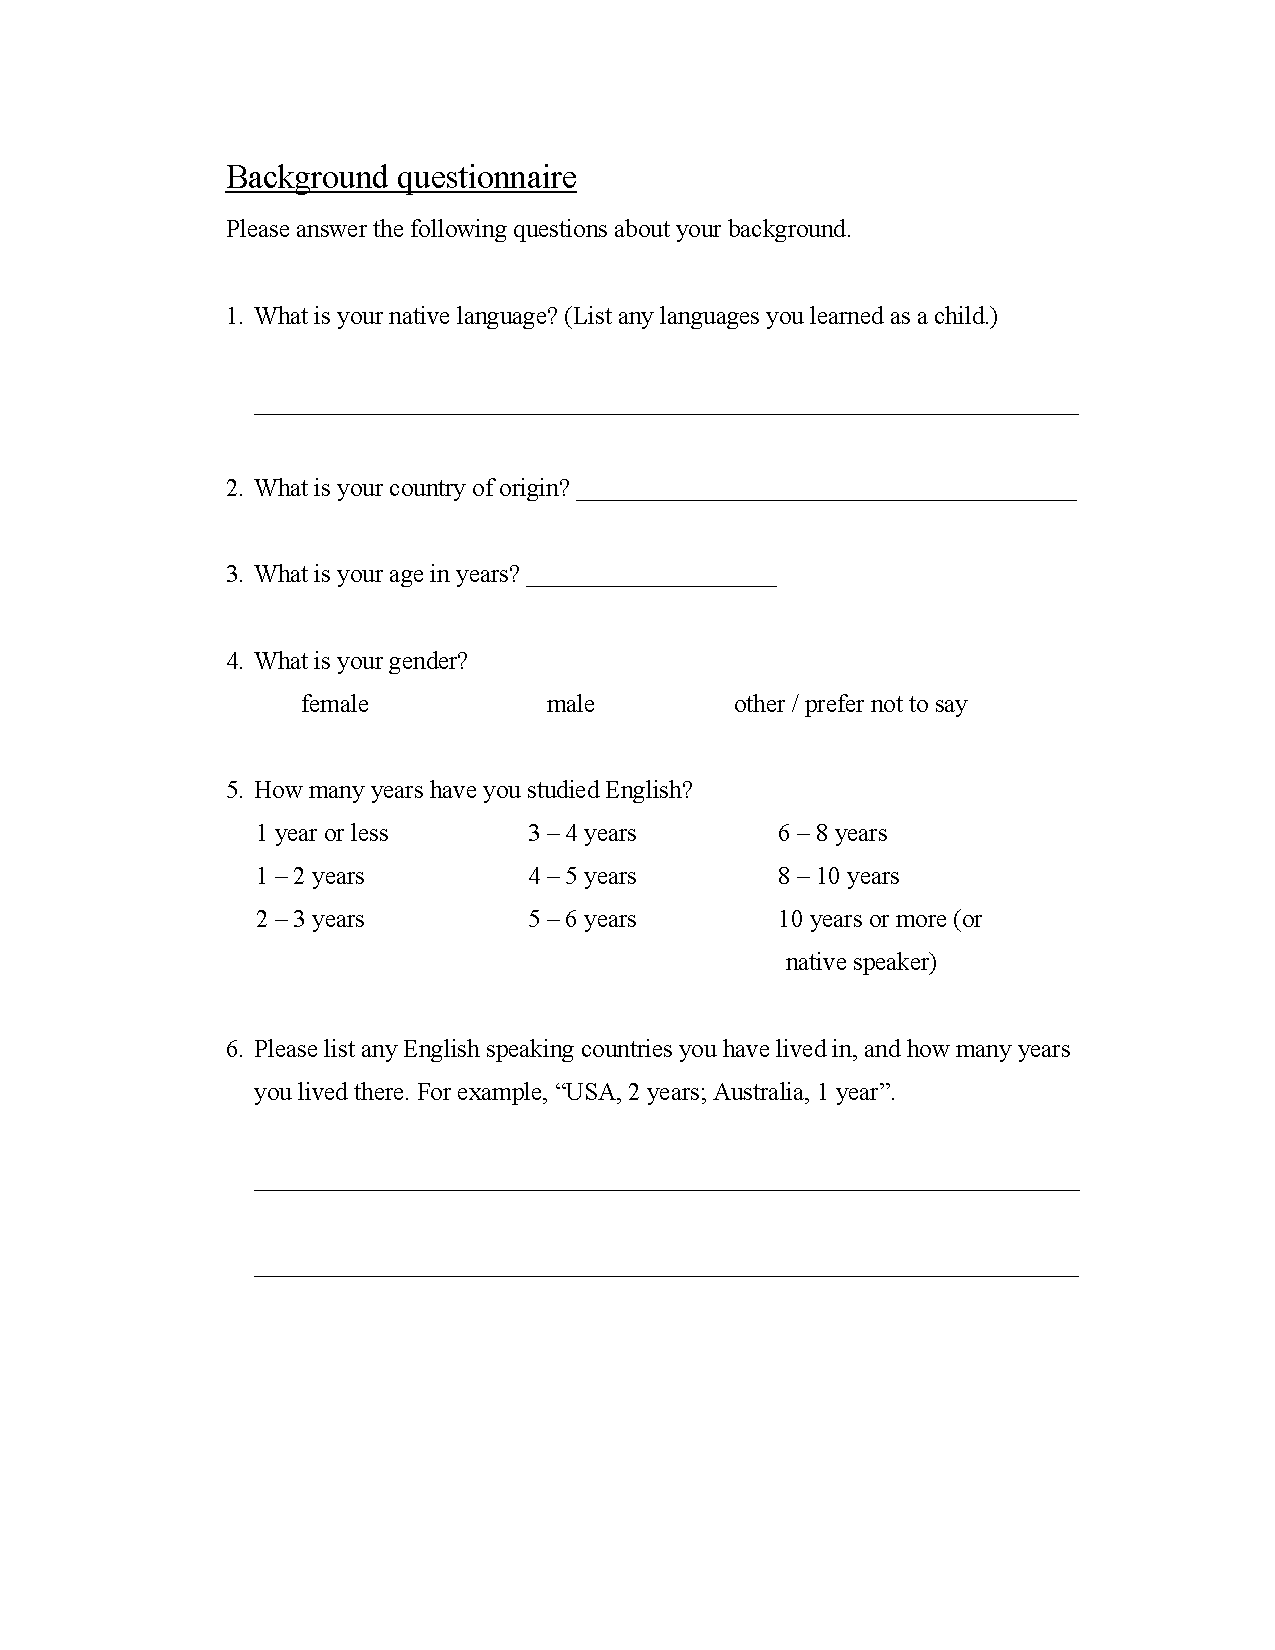
\includepdf[pages=-]{PDT_questionnaire.pdf}

\chapter{PDT Items}
\label{appendix:PDT_items}
The 30 picture description task (PDT) items are shown in this section. Each is displayed with its \textit{targeted} prompt. For all items, the \textit{untargeted} prompt is ``What is happening?'' Each item is marked as \textit{In}, \textit{Tr}, or \textit{Di} to denote it as either \textit{intransitive}, \textit{transitive}, or \textit{ditransitive}.

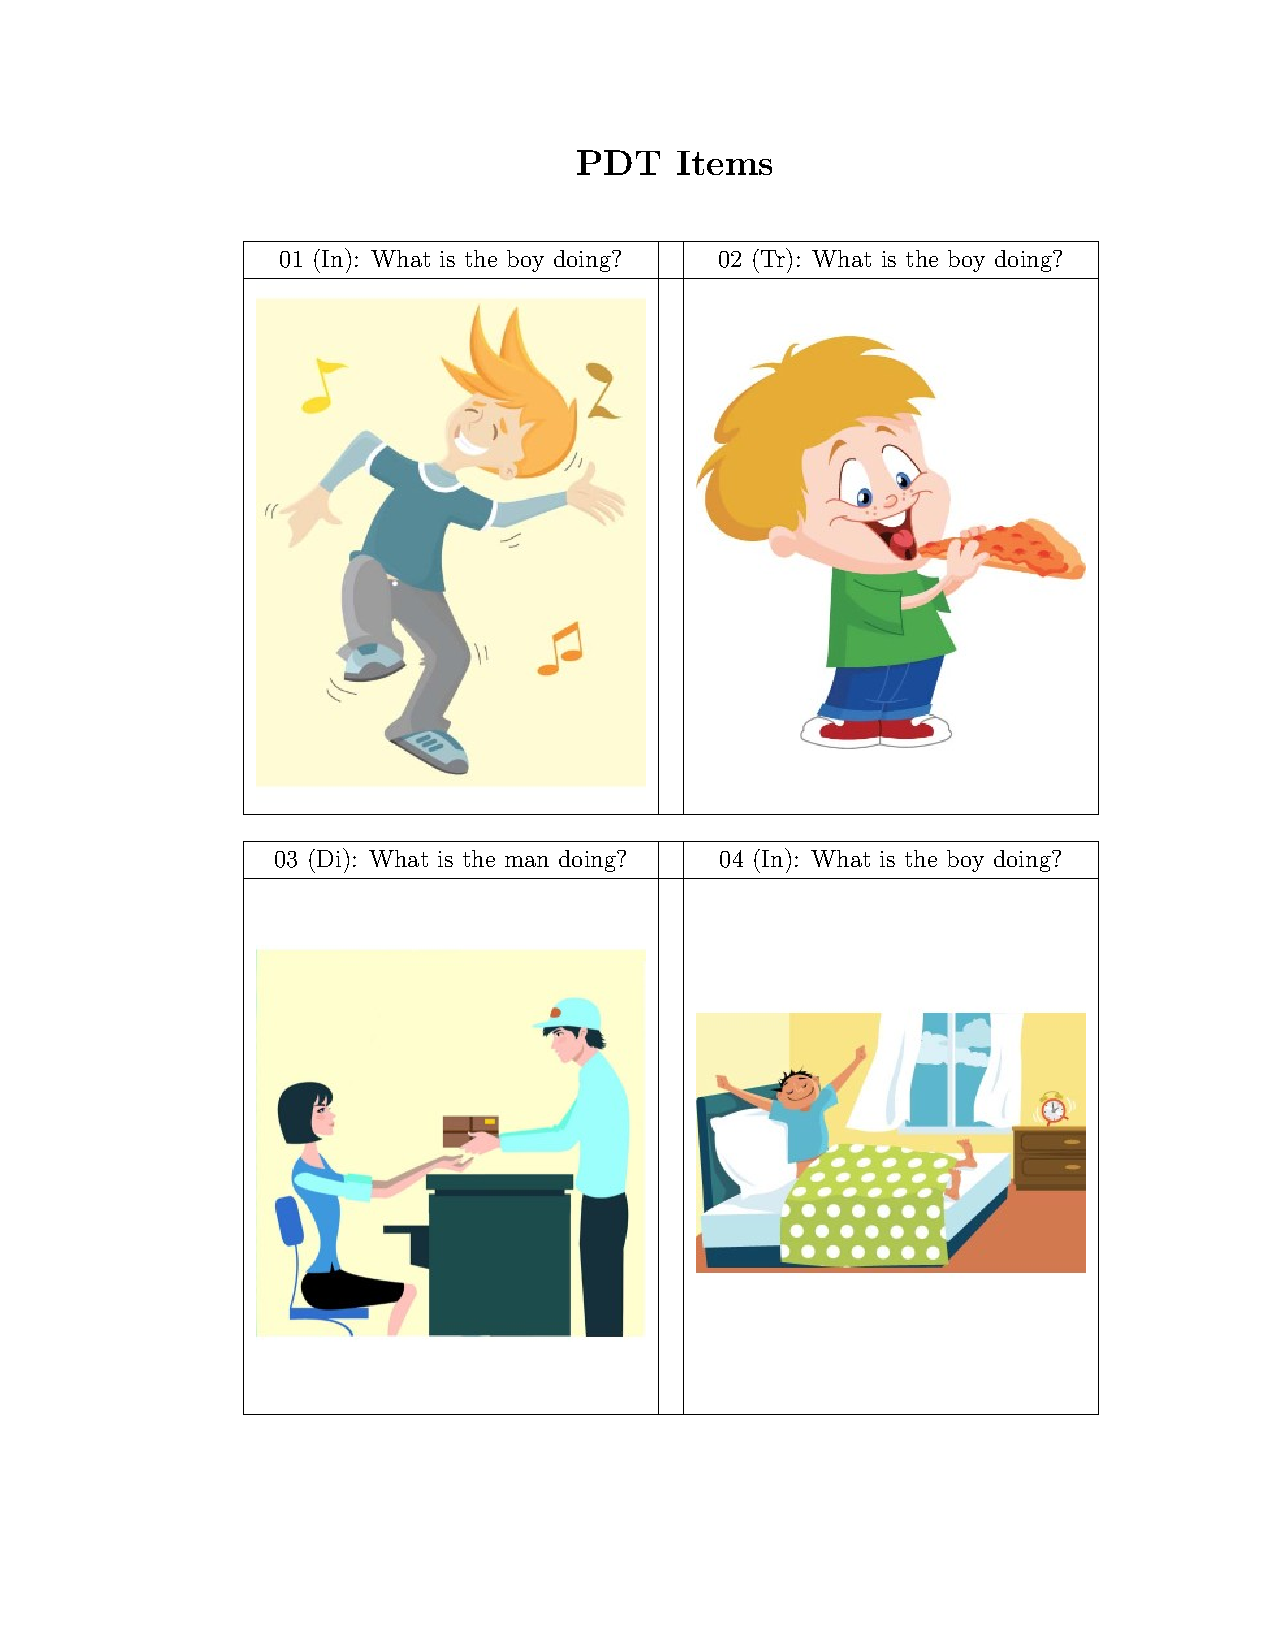
\includepdf[pages=-]{PDT_items_appendix_diss_format.pdf}

\chapter{Annotation Guide}
\label{appendix:annotation_guide}
The following pages consist of the annotation guide. This guide was produced through an iterative process of annotation and discussion between the researchers, annotators and outside linguists. This is the final version of the guidelines, which was used to produce the annotations included in the SAILS Corpus.

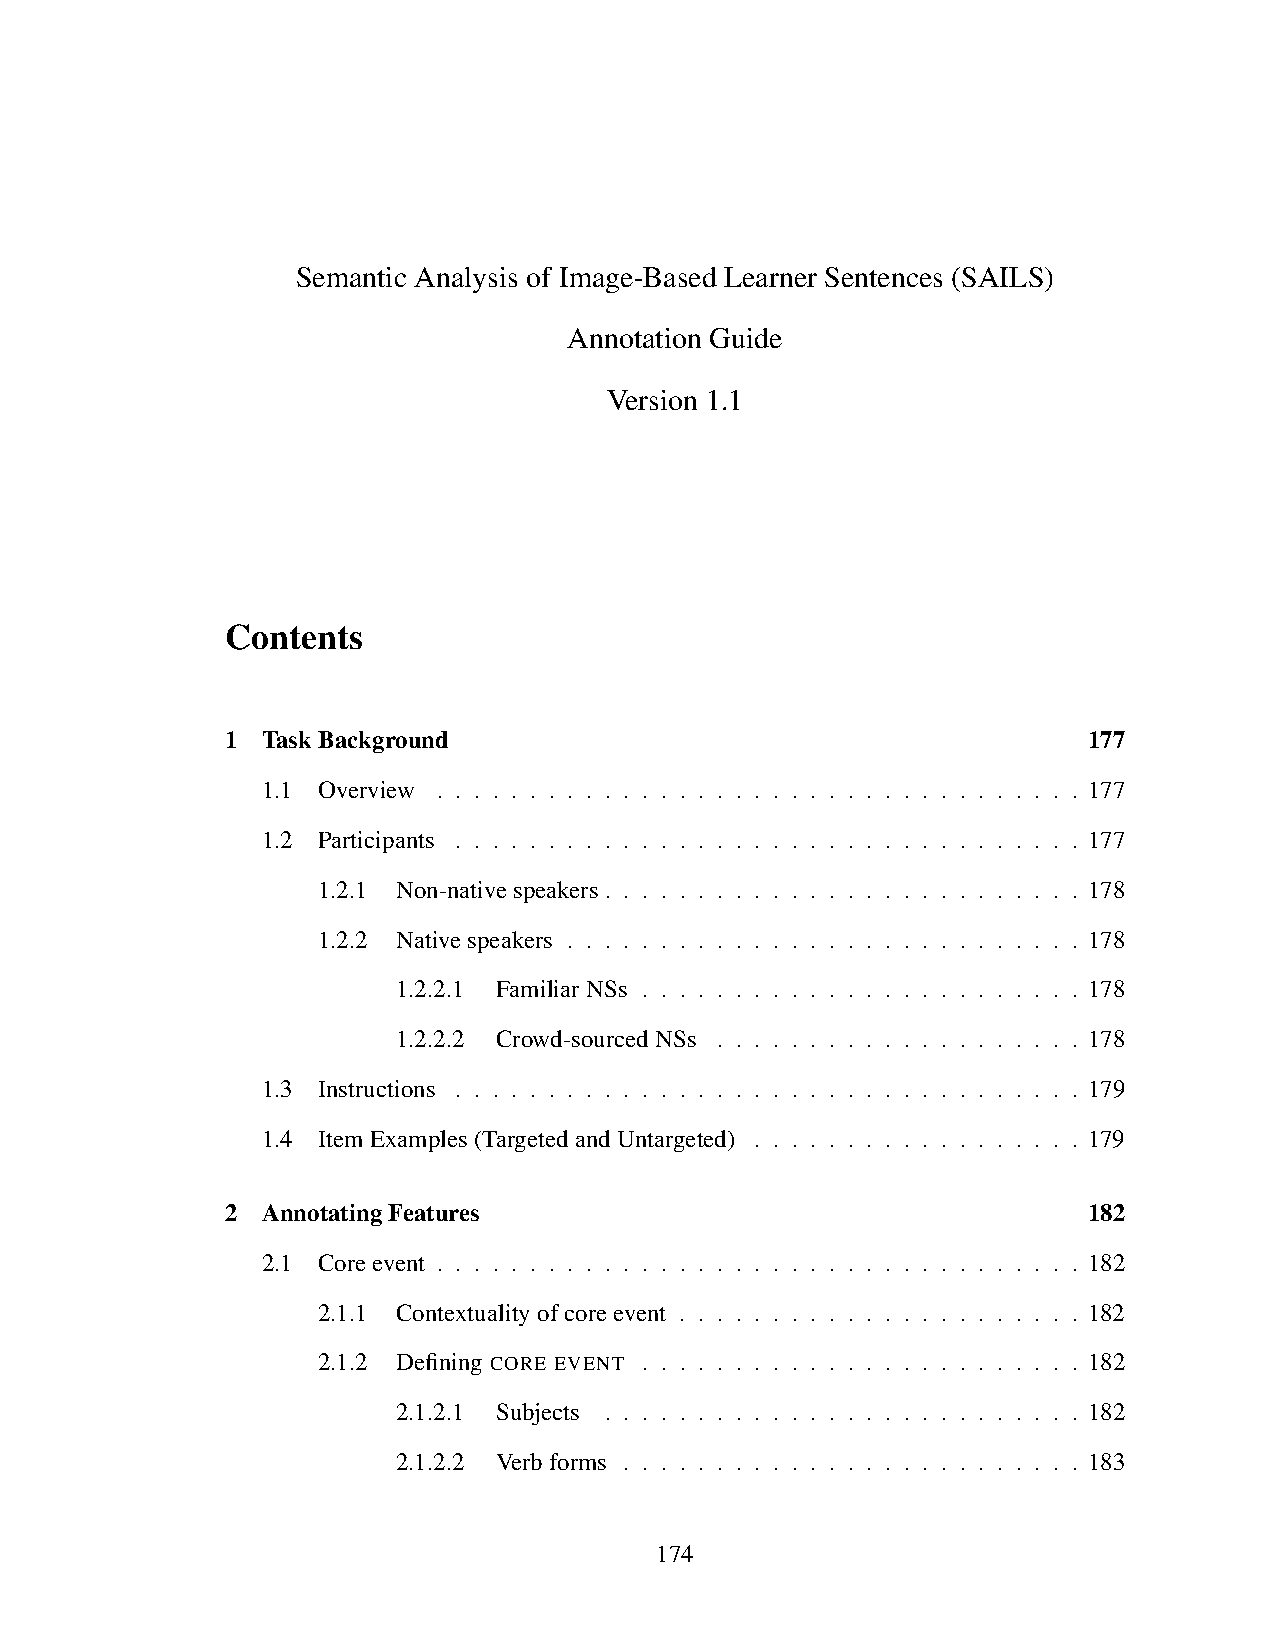
\includepdf[pages=-]{Annotation_Guide_Diss_Style.pdf}

\end{appendices}